\chapter{Gamification Analysis of Language Learning Applications}

Gamification is defined as "the use of game design elements in non-game contexts" \cite{cite:deterding2011_gamefulness}. In educational settings, it enhances learning activities through game mechanics to increase student engagement and motivation. The field encompasses numerous concepts, including streaks, achievements, leaderboards, progress tracking, social elements, virtual currencies, and much more \cite{cite:govender2021_gamification_elements_in_language_learning_apps}.

Traditional vocabulary learning methods often rely on mechanical repetition or passive reading, which can lead to decreased engagement and compromised learning outcomes. This challenge is particularly evident in language acquisition, where consistent practice is crucial for long-term retention. Gamification addresses these limitations by incorporating structured incentives for regular practice while maintaining learner engagement through various game mechanics.

While gamification offers numerous potential elements for implementation, this analysis focuses specifically on features that enhance vocabulary learning effectiveness. This chapter first examines the current gamification features in English Mind, identifying areas for potential enhancement. It then analyzes three prominent language learning applications — WordUp \cite{cite:wordup}, DuoCards \cite{cite:duocards}, and Duolingo \cite{cite:duolingo} — selected based on either their similarity to English Mind's learning approach or their innovative implementation of gamification elements. The chapter concludes with a comparative analysis of these applications and identifies key opportunities for improvement.\newpage

\section{English Mind}

English Mind currently implements minimal gamification features, consisting primarily of two basic progress visualization elements:

\begin{itemize}
    \item \textbf{Vocabulary Progress Overview} 
    \label{chap:em-progess-tracking}
    
    The application provides quantitative metrics of vocabulary acquisition progress, displaying the number of known words, words in active learning, and remaining words to be learned (see Figure \ref{fig:em-progress-tracking}). This statistical overview enables users to track their overall learning trajectory.

    \begin{figure}[!h]
        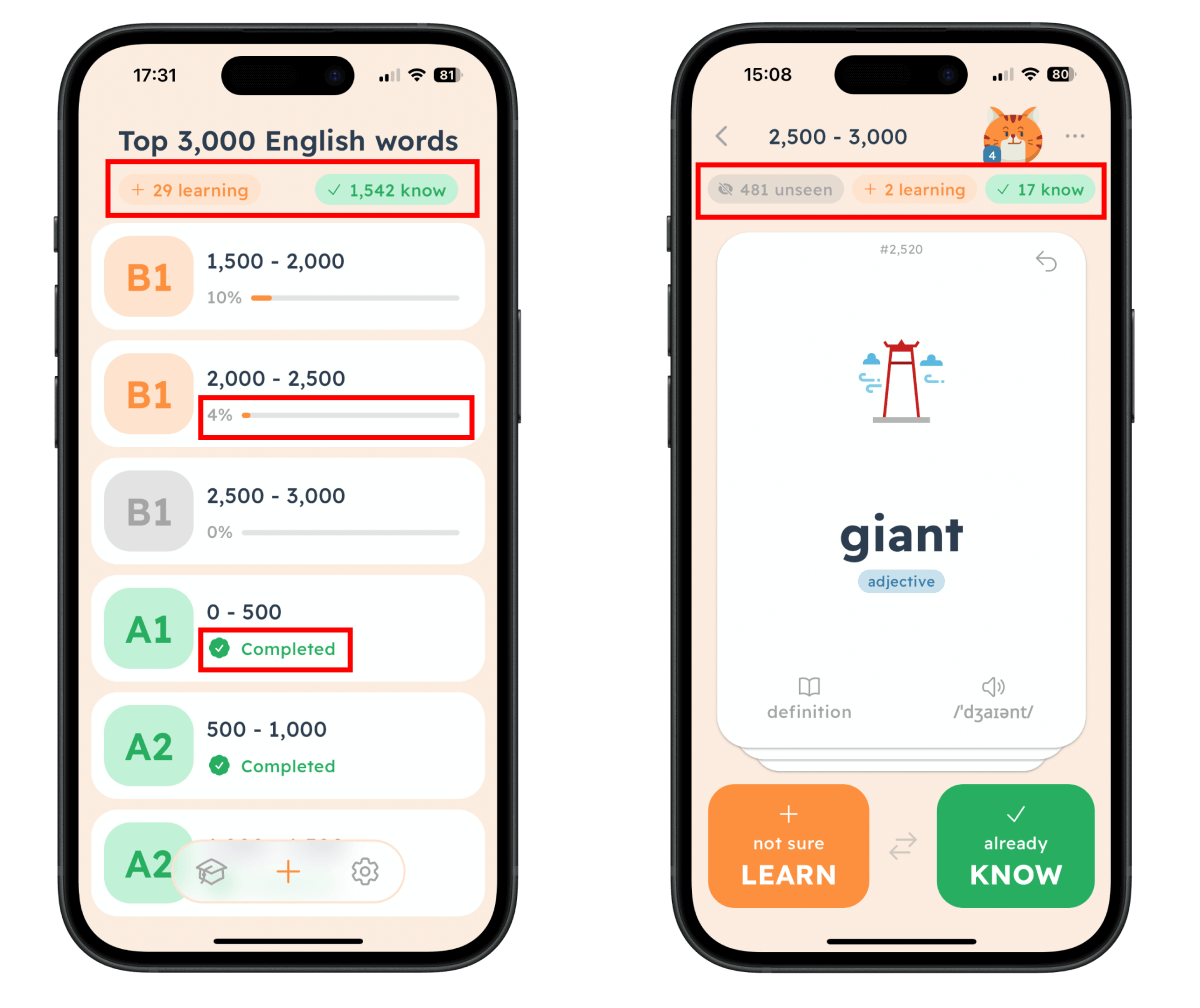
\includegraphics[width=0.9\textwidth]{src/figures/em-progress-tracking.png}
        \caption{English Mind - Vocabulary Progress Overview}
        \label{fig:em-progress-tracking}
    \end{figure}

    \item \textbf{Session Progress Indicator}
    
    A linear progress indicator during flashcard practice sessions provides visual feedback on session completion status. This basic implementation offers immediate context for session progress.
    
\end{itemize}

This limited implementation of gamification elements suggests significant potential for enhancement through more sophisticated engagement mechanisms, which will be examined through comparative analysis in subsequent sections.

\section{WordUp}

WordUp represents a particularly relevant case study as it shares the core learning methodologies with English Mind, combining frequency lists with spaced repetition and flashcard-based practice. With over 5 million downloads on Google Play \cite{cite:wordup_google_play}, its implementation of gamification elements provides comparative insights for potential enhancements to English Mind. The application implements three key gamification features:

\begin{itemize}
    \item \textbf{Diversified Flashcard Types}

    WordUp employs four variants of flashcards, each targeting different aspects of vocabulary acquisition (see Figure \ref{fig:wordup-flashcard-types}). This variation in exercise types helps maintain engagement while addressing multiple aspects of language acquisition — meaning comprehension, recall, spelling accuracy, and listening skills.
    
    \begin{itemize}
        \item Word-to-Definition matching
        \item Definition-to-Word recall
        \item Definition-to-Spelling association
        \item Audio-to-Spelling transcription
    \end{itemize}

    \begin{figure}[!h]
        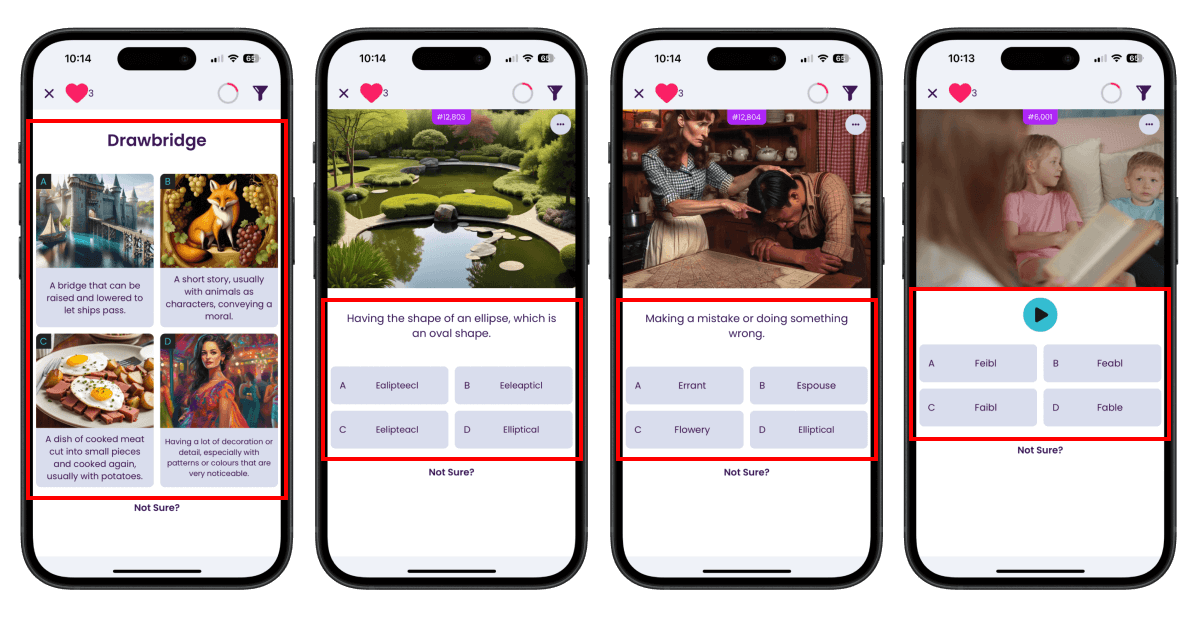
\includegraphics[width=1\textwidth]{src/figures/wordup-flashcard-types.png}
        \caption{WordUp - Flashcard Type Variations}
        \label{fig:wordup-flashcard-types}
    \end{figure}
    
    \item \textbf{Individual Word Progress Tracking}
    \label{sec:wordup-individual-word-progress-experience}
    
    The application implements a granular progress tracking system that visualizes individual word mastery through a numerical indicator (see Figure \ref{fig:wordup-word-progress}). This mechanism provides immediate feedback on learning progress at the word level.

    \begin{figure}[!h]
        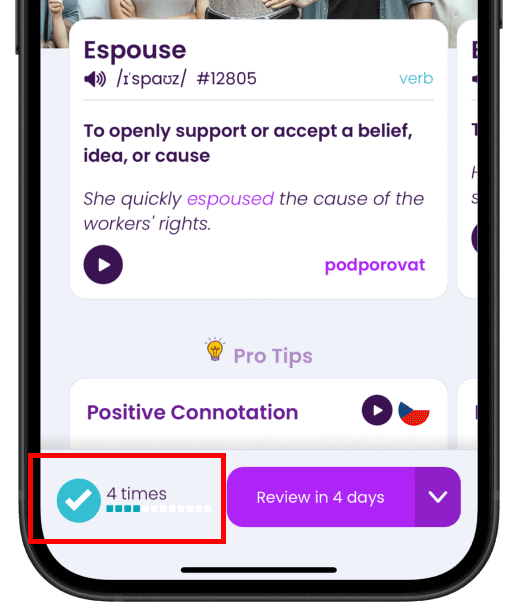
\includegraphics[width=0.35\textwidth]{src/figures/wordup-word-progress.png}
        \caption{WordUp - Individual Word Progress Indicator}
        \label{fig:wordup-word-progress}
    \end{figure}

    \item \textbf{Time-Based Goals and Social Competition}

    The application incorporates daily practice goals measured in minutes, complemented by a leaderboard system (see Figure \ref{fig:wordup-daily-goal}). This combination of personal goals and social comparison creates multiple motivation vectors for sustained engagement.

    \begin{figure}[!h]
        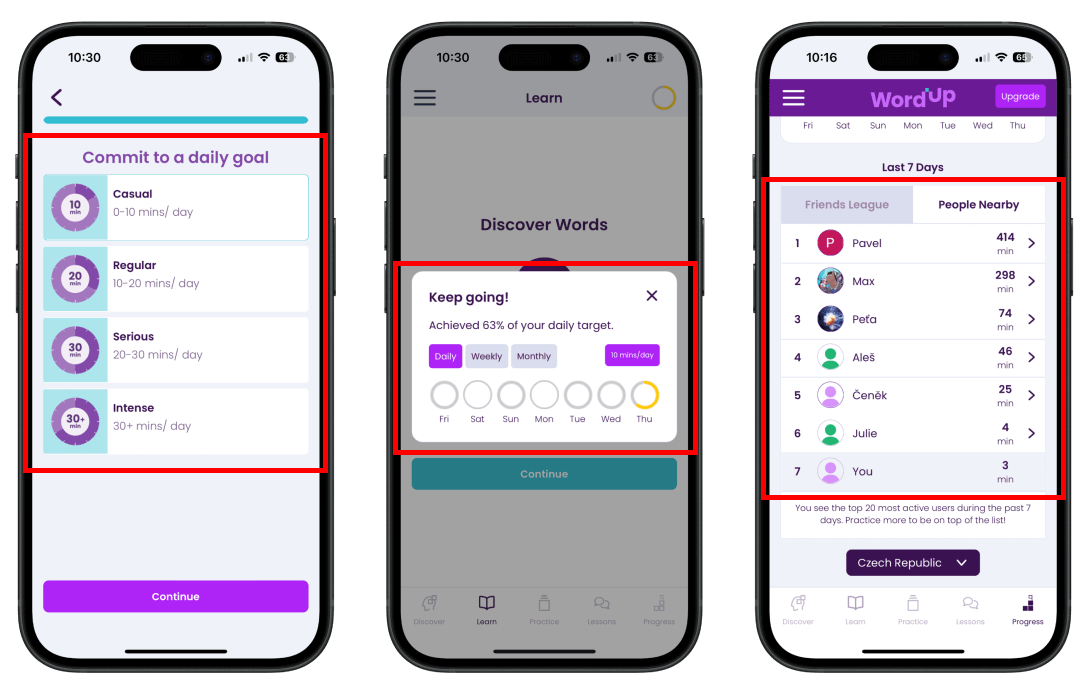
\includegraphics[width=0.99\textwidth]{src/figures/wordup-daily-goal.png}
        \caption{WordUp - Daily Goal and Leaderboard}
        \label{fig:wordup-daily-goal}
    \end{figure}

\end{itemize}

\section{DuoCards}

DuoCards, with over a million downloads on Google Play \cite{cite:duocards_google_play}, implements an SRS-based flashcard system for vocabulary acquisition. The application's gamification strategy centers on two primary mechanisms: diversified practice formats and an incentive-based progression system.

\begin{itemize}
    \item \textbf{Diversified Practice Formats}

    The application implements four distinct flashcard variants that systematically address different aspects of vocabulary acquisition (see Figure \ref{fig:duocards-flashcard-types}). This methodological variation facilitates comprehensive vocabulary acquisition while maintaining engagement through task diversity.

    \begin{itemize} 
         \item Bidirectional translation exercises
         \item Auditory comprehension and pronunciation exercises
         \item Multi-item matching exercises for vocabulary reinforcement
    \end{itemize}

    \begin{figure}[!h]
        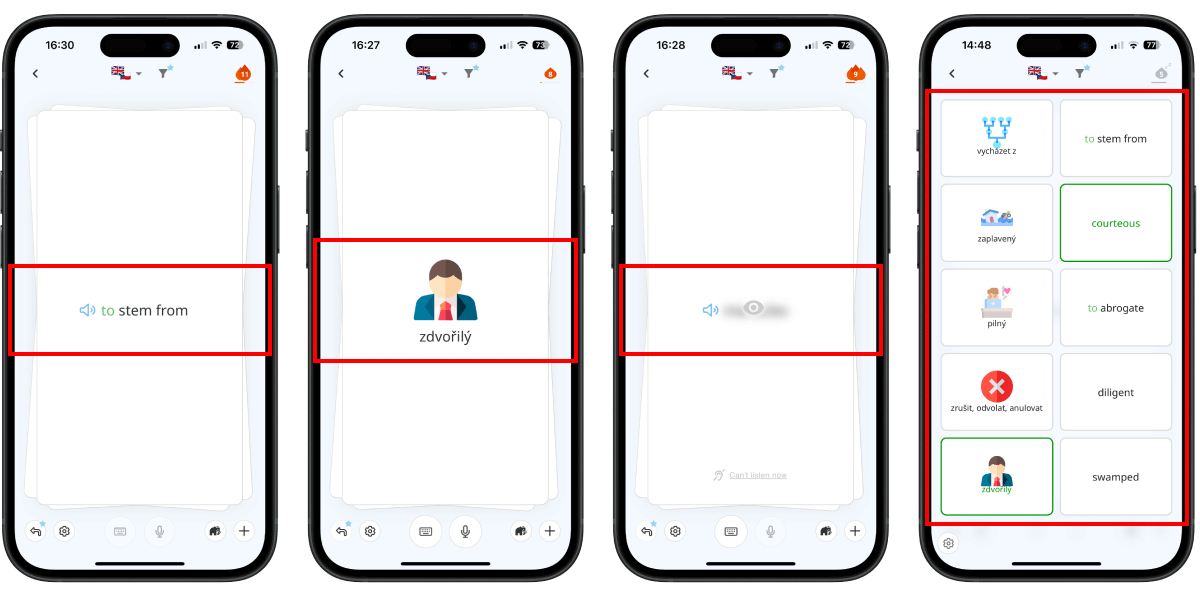
\includegraphics[width=0.98\textwidth]{src/figures/duocards-flashcard-types.png}
        \caption{DuoCards - Variation in Practice Formats}
        \label{fig:duocards-flashcard-types}
    \end{figure}
    
    \item \textbf{Virtual Currency and Achievement System}

    The application implements an experience-based reward system (XP) integrated with a customizable mascot interface (see Figure \ref{fig:duocards-memo}). This gamification mechanism creates a tangible reward structure where practice completion and vocabulary acquisition yield currency for environmental customization, thereby reinforcing consistent engagement patterns.

    \begin{figure}[!h]
        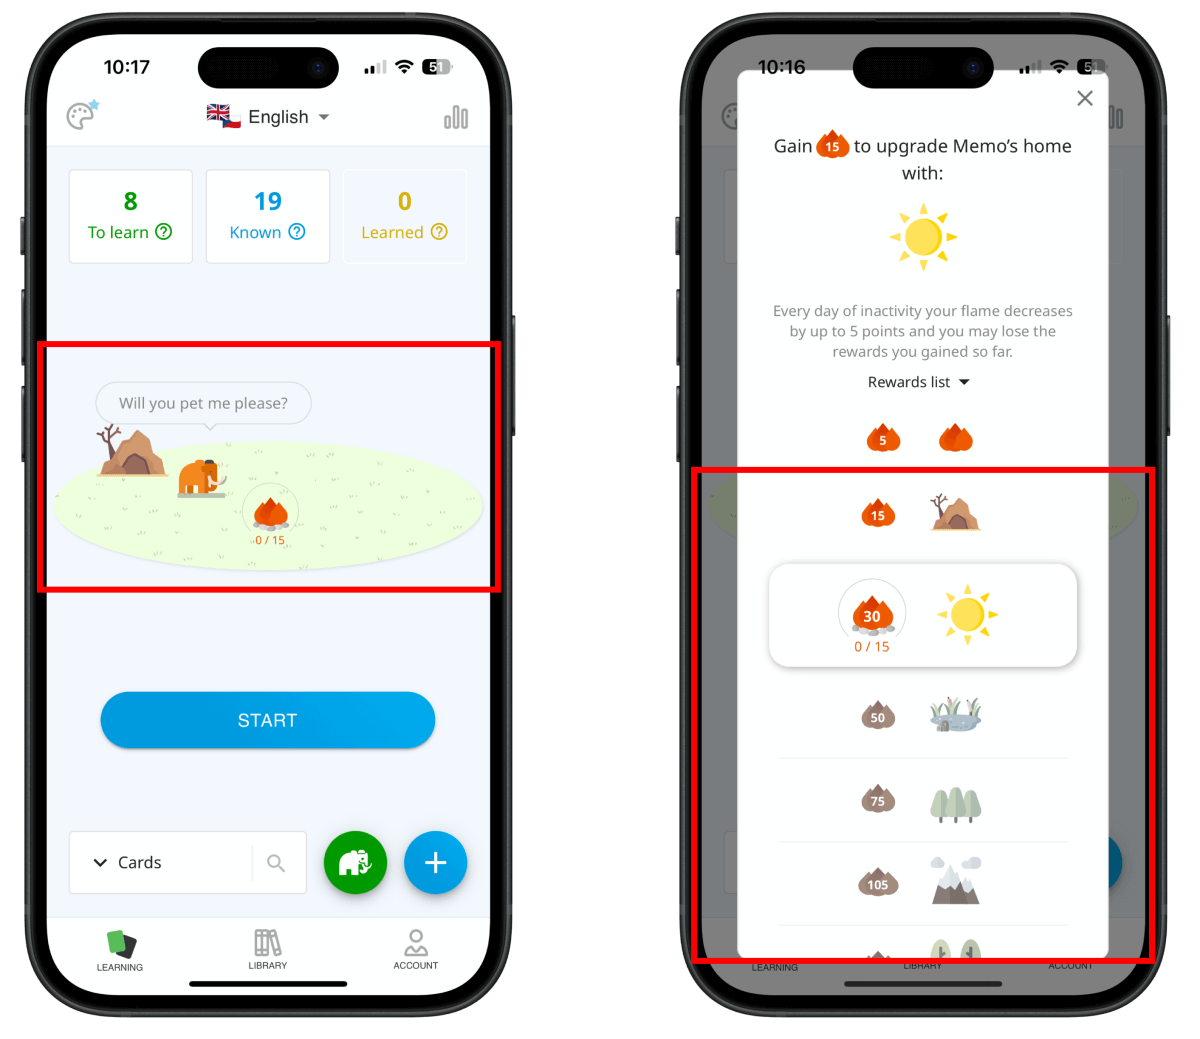
\includegraphics[width=0.7\textwidth]{src/figures/duocards-memo.png}
        \caption{DuoCards - Achievement-Based Customization}
        \label{fig:duocards-memo}
    \end{figure}

\end{itemize}

\section{Duolingo}

Duolingo, with over 100 million monthly active users \cite{cite:duolingo_2024q2}, has established significant precedent in digital language education gamification. While extensive research exists on Duolingo's comprehensive feature set, this analysis focuses on three key elements particularly relevant to English Mind's vocabulary learning context.

\begin{itemize}
    \item \textbf{Exercise Diversification}

    The application implements multiple exercise variants to reinforce vocabulary acquisition. This methodological variation addresses multiple aspects of language acquisition while maintaining engagement through task diversity (see Figure \ref{fig:duolingo-exercise-types}).

    \begin{itemize}
        \item Word-translation pair matching exercises
        \item Speech recognition-based pronunciation assessment
        \item Audio-to-text transcription for listening comprehension
    \end{itemize}

    \begin{figure}[!h]
        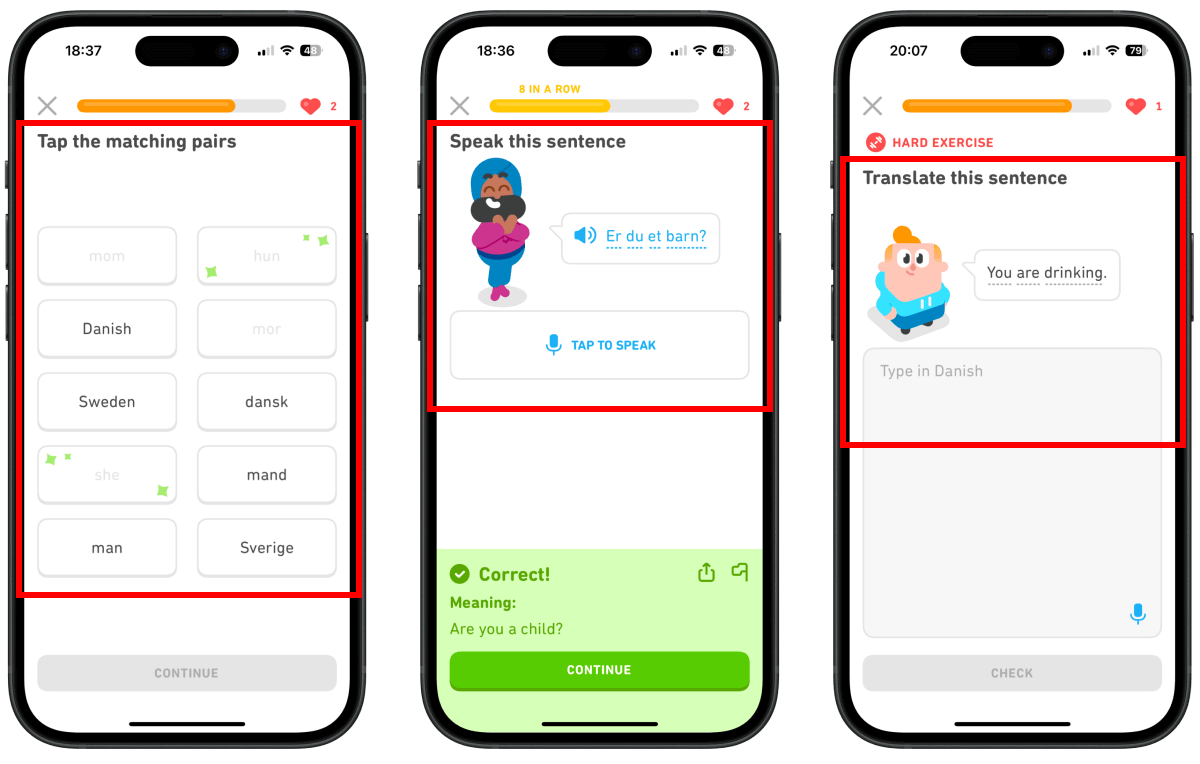
\includegraphics[width=0.9\textwidth]{src/figures/duolingo-exercise-types.png}
        \caption{Duolingo - Exercise Types}
        \label{fig:duolingo-exercise-types}
    \end{figure}
    \newpage
    \item \textbf{Post-Session Analytics}
    \label{sec:duolingo-lesson-review}

    The application provides immediate post-session feedback through quantitative metrics. This feedback mechanism facilitates progress tracking while reinforcing achievement through immediate performance visualization (see Figure \ref{fig:duolingo-lesson-review}).
    
    \begin{itemize}
        \item Performance accuracy
        \item Experience points acquired
        \item Time investment
        \item Streak metrics
    \end{itemize}

    \begin{figure}[!h]
        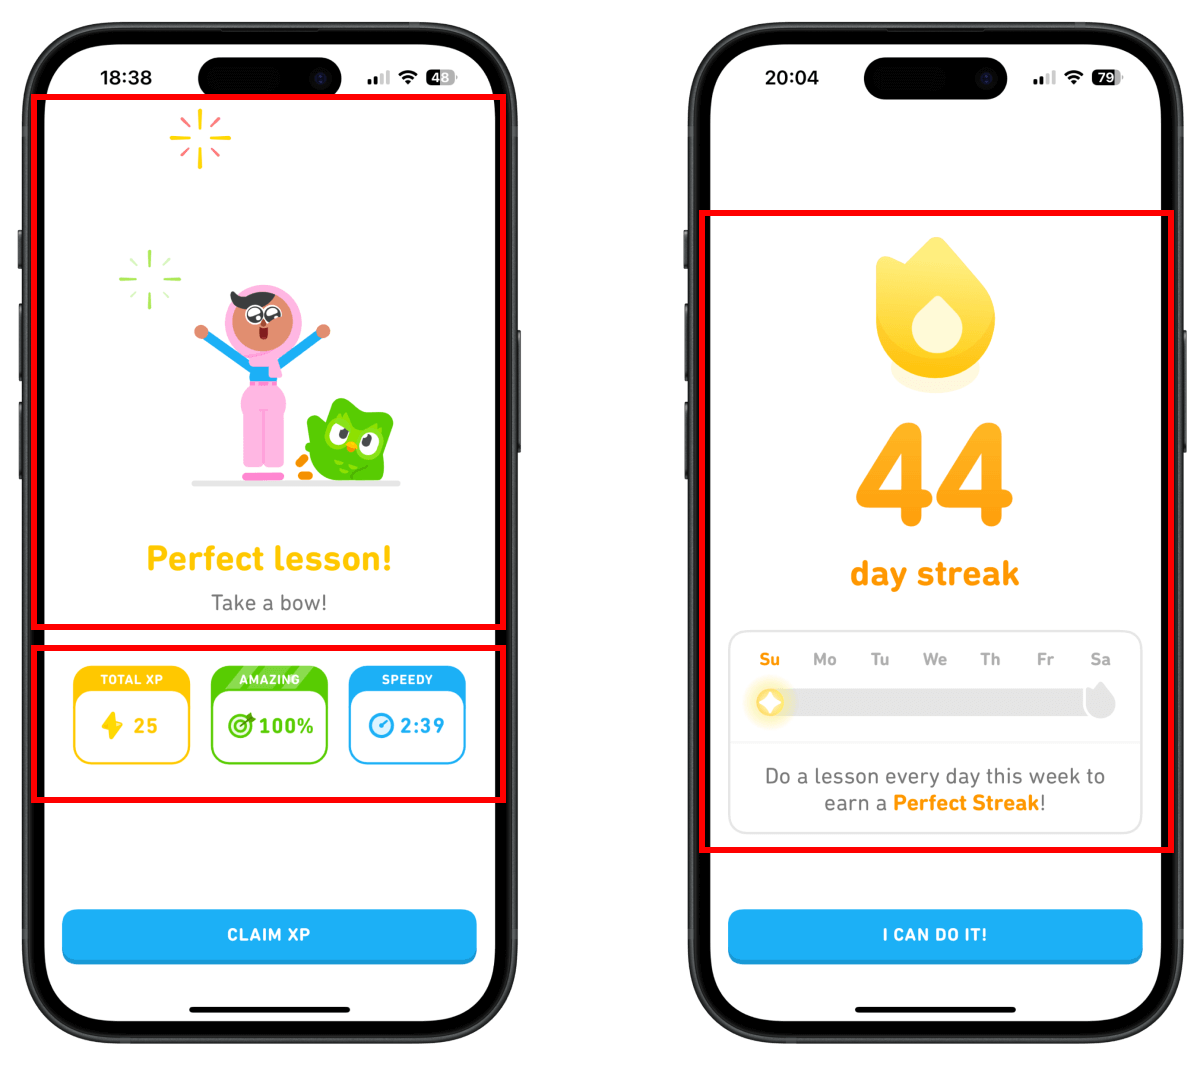
\includegraphics[width=0.8\textwidth]{src/figures/duolingo-lesson-review.png}
        \caption{Duolingo - Post-Session Analytics}
        \label{fig:duolingo-lesson-review}
    \end{figure}

    \item \textbf{Streak System}
    \label{sec:duolingo-streak-system}

    The application implements a streak-based tracking mechanism that incentivizes daily engagement. This system includes flexibility features ("Streak Freezes") to accommodate occasional missed sessions while maintaining motivation. The effectiveness is demonstrated by retention metrics, with 20\% of daily active users maintaining streaks exceeding one year \cite{cite:duolingo_2024q2}. The system is supported by a structured notification framework incorporating:
    
    \begin{itemize}
        \item Streak maintenance alerts
        \item Customizable practice reminders
        \item Achievement milestone recognition
    \end{itemize}

    \begin{figure}[!h]
        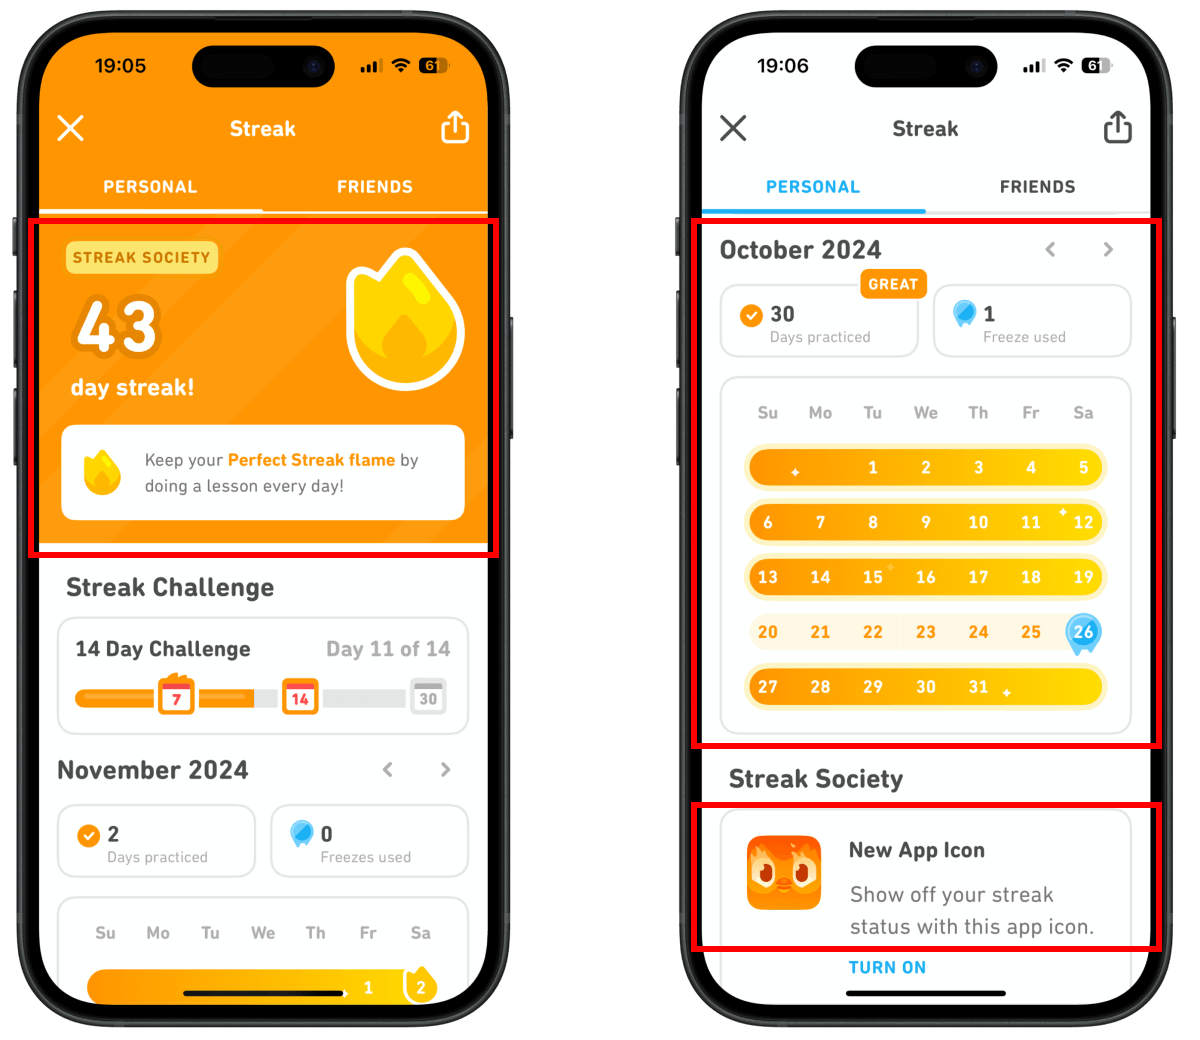
\includegraphics[width=0.8\textwidth]{src/figures/duolingo-streak.png}
        \caption{Duolingo - Streak System}
        \label{fig:duolingo-daily-streak}
    \end{figure}
\end{itemize}

\section{Comparison and Findings}

The comparative analysis of gamification features across the examined applications reveals distinct patterns in implementation approaches and feature adoption (Table \ref{tab:gamification-comparison}). The analysis yields three primary findings:
\begin{enumerate}
    \item Multiple exercise formats emerge as an industry standard, with WordUp, DuoCards, and Duolingo each implementing at least three distinct practice types. This contrasts with English Mind's single-format approach. The prevalence of varied exercise types suggests their effectiveness in both engagement and comprehensive vocabulary acquisition.

    \item Progress visualization implementations vary in granularity. While all applications provide aggregate progress metrics, WordUp's individual word progress tracking and Duolingo's post-session analytics demonstrate more sophisticated approaches to progress feedback.
    
    \item Engagement retention mechanisms vary across applications, with mainly Duolingo's streak system showing notable effectiveness.
\end{enumerate}


\begin{table}[h]
    \caption{Comparison of Gamification Features Across Applications}
    \label{tab:gamification-comparison}
    
    % Spacing between rows and columns
    \renewcommand{\arraystretch}{1.2}
    \setlength{\tabcolsep}{2pt}
    
    \begin{tabular}{l>{\centering}p{2cm}>{\centering}p{2cm}>{\centering}p{2cm}>{\centering\arraybackslash}p{2cm}}
        \toprule
        \textbf{Feature} & \textbf{English Mind} & \textbf{WordUp} & \textbf{DuoCards} & \textbf{Duolingo} \\
        \midrule
        \multicolumn{5}{l}{\textbf{Flashcard Variations}} \\
        Multiple flashcard types & \textemdash & \ding{51} & \ding{51} & \ding{51} \\
        Spelling exercises & \textemdash & \ding{51} & \ding{51} & \ding{51} \\
        Matching exercises & \textemdash & \ding{51} & \ding{51} & \ding{51} \\
        Speaking exercises & \textemdash & \textemdash & \textemdash & \ding{51} \\
        \midrule
        \multicolumn{5}{l}{\textbf{Progress Tracking}} \\
        Overall progress visualization & \ding{51} & \ding{51} & \ding{51} & \ding{51} \\
        Practice session progress bar & \ding{51} & \ding{51} & \ding{51} & \ding{51} \\
        Individual word progress & \textemdash & \ding{51} & \textemdash & \textemdash \\
        \midrule
        \multicolumn{5}{l}{\textbf{Streaks and Daily Goals}} \\
        Streak system & \textemdash & \textemdash & \ding{51} & \ding{51} \\
        Daily word goal & \ding{51} & \textemdash & \textemdash & \textemdash \\
        Daily time goal & \textemdash & \ding{51} & \textemdash & \textemdash \\
        \midrule
        \multicolumn{5}{l}{\textbf{Rewards and Motivation}} \\
        Virtual currency & \textemdash & \textemdash & \ding{51} & \ding{51} \\
        Post-practice review & \textemdash & \textemdash & \textemdash & \ding{51} \\ 
        Leaderboards & \textemdash & \ding{51} & \textemdash & \ding{51} \\
        Mascot upgrade system & \textemdash & \textemdash & \ding{51} & \textemdash \\
        \bottomrule
    \end{tabular}
\end{table}